\chapter{\textit{PeleC} Input Parameters for Simulations} \label{Pelec-Inputs}
Here inputs are provided to aid in reproducibility of the present simulations. Note though that the current version of \textit{PeleC} may have different input structures compared to those displayed here. The following git hashes were used for this work:

PeleC git hash: v0.1-130-gd489031-dirty

AMReX git hash: 19.06-406-ge73f42267

PelePhysics git hash: v0.1-16-g64d0135

\begin{figure}[H]
\begin{center}
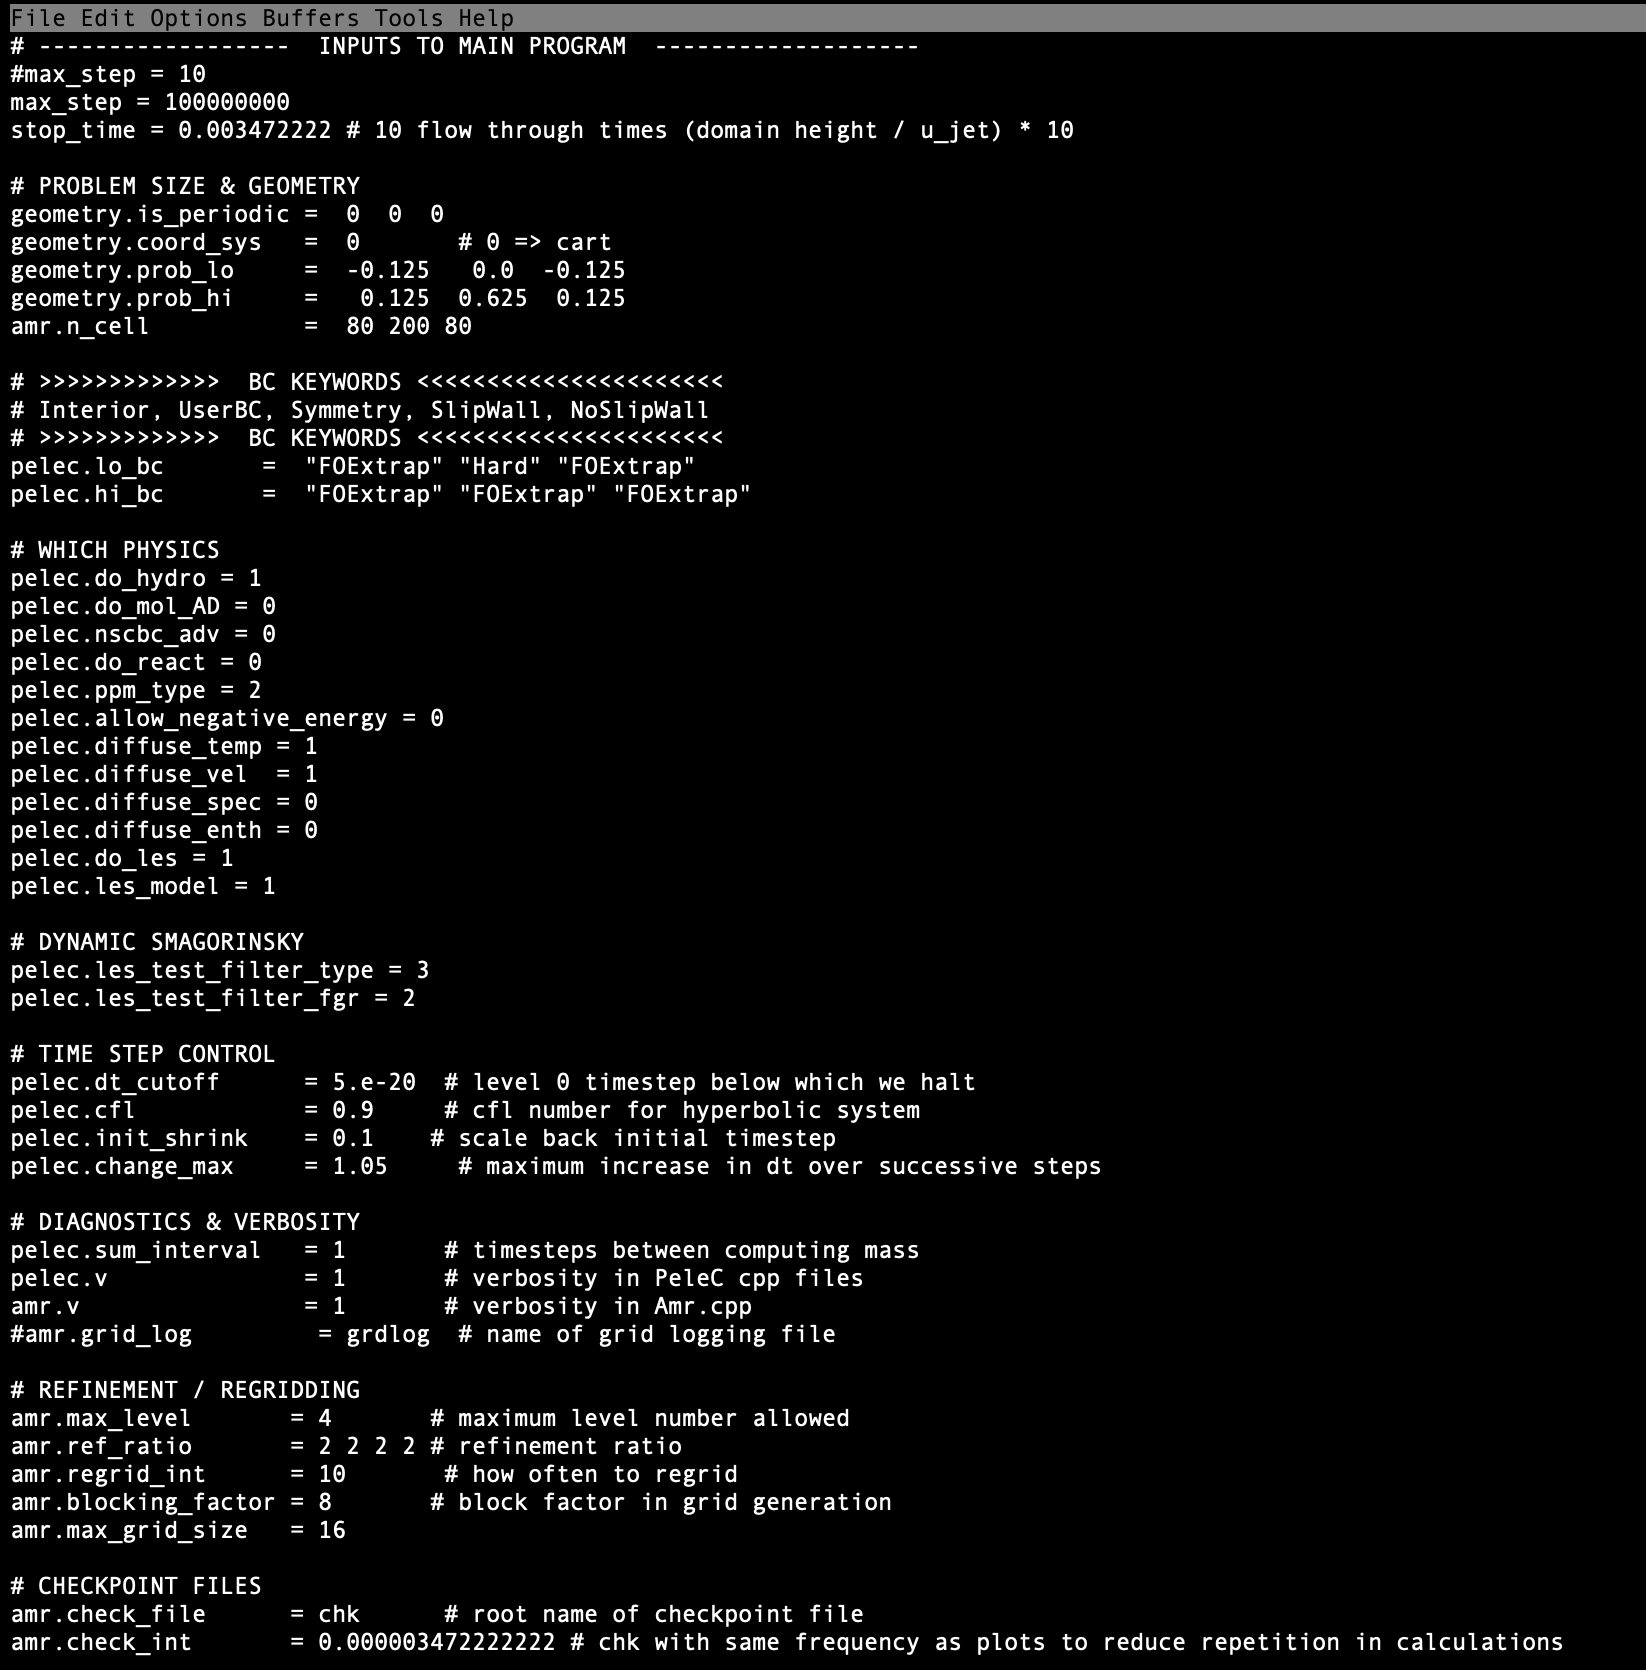
\includegraphics[scale=0.5]{figures/inputs.png}
\end{center}
\caption{Input parameters for available physics options in \text{PeleC}}
\label{PeleC_input_fig}
\end{figure} 

\begin{figure}[H]
\begin{center}
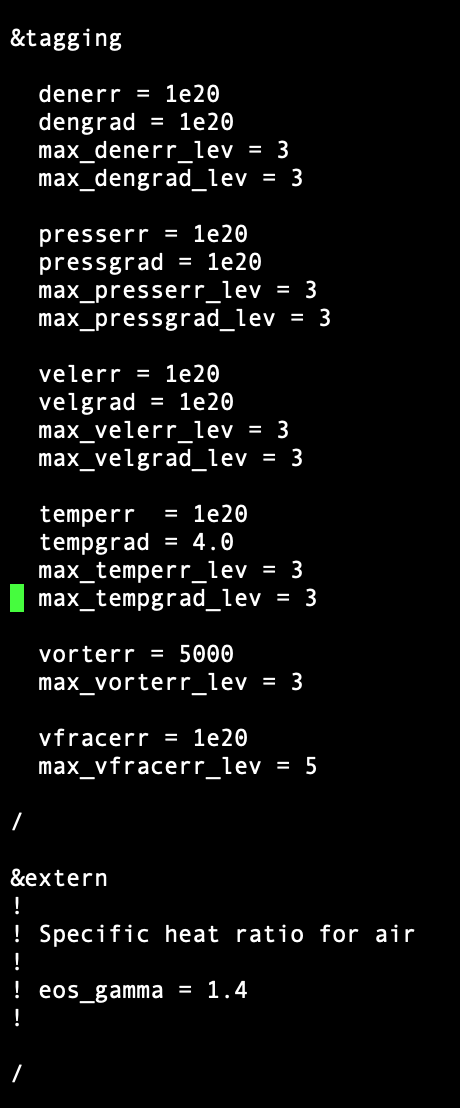
\includegraphics[scale=0.5]{figures/tagging.png}
\end{center}
\caption{AMR tagging criteria selected within in \text{PeleC}}
\label{PeleC_tagging_fig}
\end{figure} 